\documentclass[12pt]{article}
%%%%%%%%%%%%%%%%
% Packages
%%%%%%%%%%%%%%%%

\usepackage[top=2cm,bottom=2cm,left=2cm,right= 2cm]{geometry}
\usepackage[parfill]{parskip}
\usepackage{graphicx, fontspec, xcolor,multicol, enumitem, setspace, amsmath, changepage}
\DeclareGraphicsRule{.tif}{png}{.png}{`convert #1 `dirname #1`/`basename #1 .tif`.png}

%%%%%%%%%%%%%%%%
% User defined colors
%%%%%%%%%%%%%%%%

% Pantone 2015 Fall colors
% http://iwork3.us/2015/02/18/pantone-2015-fall-fashion-report/
% update each semester or year

\xdefinecolor{custom_blue}{rgb}{0, 0.32, 0.48} % FROM SPRING 2016 COLOR PREVIEW
\xdefinecolor{custom_darkBlue}{rgb}{0.20, 0.20, 0.39} % Reflecting Pond  
\xdefinecolor{custom_orange}{rgb}{0.96, 0.57, 0.42} % Cadmium Orange
\xdefinecolor{custom_green}{rgb}{0, 0.47, 0.52} % Biscay Bay
\xdefinecolor{custom_red}{rgb}{0.58, 0.32, 0.32} % Marsala

\xdefinecolor{custom_lightGray}{rgb}{0.78, 0.80, 0.80} % Glacier Gray
\xdefinecolor{custom_darkGray}{rgb}{0.35, 0.39, 0.43} % Stormy Weather

%%%%%%%%%%%%%%%%
% Color text commands
%%%%%%%%%%%%%%%%

%orange
\newcommand{\orange}[1]{\textit{\textcolor{custom_orange}{#1}}}

% yellow
\newcommand{\yellow}[1]{\textit{\textcolor{yellow}{#1}}}

% blue
\newcommand{\blue}[1]{\textit{\textcolor{blue}{#1}}}

% green
\newcommand{\green}[1]{\textit{\textcolor{custom_green}{#1}}}

% red
\newcommand{\red}[1]{\textit{\textcolor{custom_red}{#1}}}

%%%%%%%%%%%%%%%%
% Coloring titles, links, etc.
%%%%%%%%%%%%%%%%

\usepackage{titlesec}
\titleformat{\section}
{\color{custom_blue}\normalfont\Large\bfseries}
{\color{custom_blue}\thesection}{1em}{}
\titleformat{\subsection}
{\color{custom_blue}\normalfont}
{\color{custom_blue}\thesubsection}{1em}{}

\newcommand{\ttl}[1]{ \textsc{{\LARGE \textbf{{\color{custom_blue} #1} } }}}

\newcommand{\tl}[1]{ \textsc{{\large \textbf{{\color{custom_blue} #1} } }}}

\usepackage[colorlinks=false,pdfborder={0 0 0},urlcolor= custom_orange,colorlinks=true,linkcolor= custom_orange, citecolor= custom_orange,backref=true]{hyperref}

%%%%%%%%%%%%%%%%
% Instructions box
%%%%%%%%%%%%%%%%

\newcommand{\inst}[1]{
\colorbox{custom_blue!20!white!50}{\parbox{\textwidth}{
	\vskip10pt
	\leftskip10pt \rightskip10pt
	#1
	\vskip10pt
}}
\vskip10pt
}

%%%%%%%%%%%
% App Ex number    %
%%%%%%%%%%%

% DON'T FORGET TO UPDATE

\newcommand{\appno}[1]
{1.3}

%%%%%%%%%%%%%%
% Turn on/off solutions       %
%%%%%%%%%%%%%%

% Off
\newcommand{\soln}[2]{$\:$\\ \vspace{#1}}{}

%% On
%\newcommand{\soln}[2]{\textit{\textcolor{custom_red}{#2}}}{}

%%%%%%%%%%%%%%%%
% Document
%%%%%%%%%%%%%%%%

\begin{document}
\fontspec[Ligatures=TeX]{Helvetica Neue Light}

Dr. \c{C}etinkaya-Rundel \hfill Sta 101: Data Analysis and Statistical Inference \\
Duke University - Department of Statistical Science \hfill \\

\ttl{Application exercise \appno{}: \\
Scientific studies in the press}

\inst{$\:$ \\
Team name: \rule{10cm}{0.5pt} \\
$\:$ \\
Lab section: $\qquad$ 8:30 $\qquad$ 10:05 $\qquad$ 11:45 $\qquad$ 1:25 $\qquad$ 3:05 \\
$\:$ \\
Write your responses in the spaces provided below. WRITE LEGIBLY and SHOW ALL WORK! 
Only one submission per team is required. One team will be randomly selected and their 
responses will be discussed and graded. Concise and coherent are best!}

\begin{minipage}[c]{0.72\textwidth}
In this activity you will read media coverage of a study published in a peer reviewed 
journal, and answer a few of question about a study. It is possible that the article 
doesn't provide the relevant information to answer certain question(s). If so, refer 
to the original study (linked below). You do not need to read the entire paper, in fact, 
you are certainly not expected to understand all of it. Simply find the information that 
will help you answer the questions. \\

\begin{minipage}[t]{0.49\textwidth}
\textbf{Media coverage:} \\
{\small
Haters Are Gonna Hate, Study Confirms \\
By  Katy Waldman \\
Published: August 28, 2013 on Slate \\
Link: \url{http://slate.me/1dr5XPE} \\
}
\end{minipage}
\begin{minipage}[t]{0.02\textwidth}
$\:$ \\
\end{minipage}
\begin{minipage}[t]{0.49\textwidth}
\textbf{Original study:} \\
{\small
Hepler, J., \& Albarracin, D. (2013). ``Attitudes without objects: Evidence for a 
dispositional attitude, its measurement, and its consequences". \textit{Journal of 
personality and social psychology}, 104(6), 1060. \\
Link: \url{https://sakai.duke.edu/x/oIukKJ} \\
}
\end{minipage}

\end{minipage}
\begin{minipage}[c]{0.03\textwidth}
$\:$ \\
\end{minipage}
\begin{minipage}[c]{0.25\textwidth}
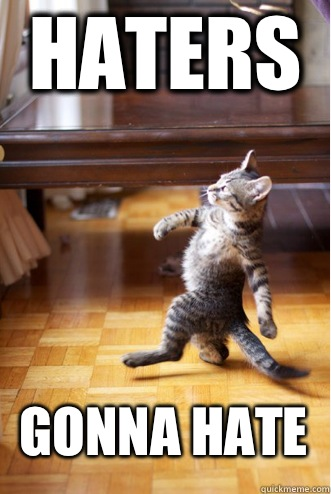
\includegraphics[width = \textwidth]{haters.jpg}
$\:$ \\
\end{minipage}

\begin{enumerate}

\item What are the cases, i.e. observations?

\soln{1cm}{200 men and women}

\item What is (are) the response variable(s) in this study?

\soln{1cm}{Attitude towards the microwave oven}

\pagebreak

\item What is (are) the explanatory variable(s) in this study?

\soln{1cm}{Whether the participant is a hater or not}

\item Does the study employ random sampling? How about random assignment?

\soln{1cm}{Via Amazon's MTurk - self selected sample, no random assignment}

\item Is this an observational study or an experiment? Explain your reasoning.

\soln{1cm}{Observational, doesn't use random assignment}

\item Can we establish a causal link between the explanatory and response variables?

\soln{1cm}{No}

\item Can the results of the study be generalized to the population at large?

\soln{1cm}{No}

\end{enumerate}



\end{document}